% =====================================================================================
% Relatório da Entrega 1 -- Proposta e Análise Exploratória dos Dados
% Formato: APA 7.ª edição (classe apa7, modo estudante) | Idioma: português do Brasil
% Compilação:  pdflatex relatorio && biber relatorio && pdflatex relatorio && pdflatex relatorio
% =====================================================================================
\documentclass[stu,a4paper,12pt,floatsintext,biblatex]{apa7}

\usepackage[utf8]{inputenc}
\usepackage[T1]{fontenc}
\usepackage[brazilian]{babel}
\usepackage{csquotes}
\usepackage{booktabs,graphicx,amsmath,amssymb,xspace,enumitem,tikz,float}
\usetikzlibrary{arrows.meta,positioning,calc,decorations.pathreplacing}

\hypersetup{hidelinks}
\setlength{\headheight}{15pt}
\graphicspath{{../figuras/}}
\DeclareLanguageMapping{brazilian}{brazilian-apa}
\addbibresource{referencias.bib}

% Rótulos em português para elementos fixos da classe apa7
\AtBeginDocument{\def\keywordname{Palavras-chave}\def\notelabel{Nota}}

% Números gerados pelos scripts (piloto, verificação) e recursos de hardware
% Gerado automaticamente por codigo/piloto_eda.py -- não editar à mão.
\newcommand{\PilotoRho}{0,90\xspace}
\newcommand{\PilotoMedia}{9,112\xspace}
\newcommand{\PilotoDp}{1,166\xspace}
\newcommand{\PilotoCv}{12,8\xspace}
\newcommand{\PilotoAssim}{1,34\xspace}
\newcommand{\PilotoShapW}{0,891\xspace}
\newcommand{\PilotoShapP}{0,005\xspace}
\newcommand{\PilotoTeo}{9,00\xspace}
\newcommand{\PilotoErro}{1,2\xspace}
\newcommand{\PilotoIcInf}{8,68\xspace}
\newcommand{\PilotoIcSup}{9,55\xspace}
\newcommand{\PilotoZeroEmp}{10,4\xspace}
\newcommand{\PilotoZeroTeo}{10\xspace}
\newcommand{\PilotoLagum}{0,99\xspace}
\newcommand{\PilotoLagdez}{0,90\xspace}
\newcommand{\PilotoPnoventa}{44,2\xspace}
\newcommand{\PilotoMaximo}{64,0\xspace}
\newcommand{\PilotoTempo}{0,45\xspace}
\newcommand{\PilotoLnAssim}{0,96\xspace}
\newcommand{\PilotoLnShapP}{0,058\xspace}
\newcommand{\RepLagum}{0,22\xspace}
\newcommand{\RepLagumP}{0,25\xspace}
\newcommand{\WelchIniMedia}{7,42\xspace}
\newcommand{\WelchPlatoMedia}{8,90\xspace}
\newcommand{\WelchDifPct}{$-$16,6\xspace}
\newcommand{\WelchResidDif}{$-$0,12\xspace}
\newcommand{\WelchResidEp}{0,36\xspace}
\newcommand{\CompCurtoCv}{17,2\xspace}
\newcommand{\CompCurtoMeia}{12,3\xspace}
\newcommand{\CompLongoCv}{12,8\xspace}
\newcommand{\CompLongoMeia}{9,2\xspace}
\newcommand{\TempoTotalEstimado}{36\xspace}
\newcommand{\NClientes}{50.000\xspace}
\newcommand{\NCurto}{10.000\xspace}
\newcommand{\Aquecimento}{1.000\xspace}
\newcommand{\RPiloto}{30\xspace}
\newcommand{\RWelch}{300\xspace}
\newcommand{\NWelch}{6.000\xspace}
\newcommand{\JanelaWelch}{250\xspace}

% Gerado por codigo/verificacao_simulador.py
\newcommand{\VerifMaxErro}{1,3\xspace}
\newcommand{\VerifNLongo}{400.000\xspace}
\newcommand{\VerifReps}{5\xspace}

% Recursos de hardware do ambiente onde o piloto foi executado.
% >>> Se as corridas finais forem executadas em outra máquina, edite estas linhas. <<<
\newcommand{\HwCPU}{Intel(R) Xeon(R) Processor @ 2.10GHz}
\newcommand{\HwNucleos}{1}
\newcommand{\HwRAM}{3,9}
\newcommand{\HwSO}{Linux 6.18.44-fc-v37}
\newcommand{\SwTeX}{pdfTeX 3.141592653-2.6-1.40.25 (TeX Live 2023/Debian)}
\newcommand{\SwBiber}{2.19}

\newcommand{\Wq}{W_q}

% ------------------------------------------------------------------------- capa
\title{Desempenho de Sistemas de Filas Simulados: Proposta de Experimento Fatorial \texorpdfstring{$2^3$}{2\textasciicircum 3} com Replicações e Análise Exploratória dos Dados}
\shorttitle{EXPERIMENTO FATORIAL EM FILAS SIMULADAS}
\authorsnames{Gruner Antonio Sanchez Morales}
\authorsaffiliations{Departamento de Computação, Universidade Federal de Ouro Preto}
\course{Projeto e Análise de Experimentos Computacionais --- Entrega 1}
\professor{\ }
\duedate{21 de setembro de 2026}

\abstract{Este relatório apresenta a proposta de um experimento computacional e a análise exploratória dos dados que o fundamenta.
O problema investigado é o efeito de três fatores --- número de servidores, taxa de chegada e distribuição do tempo de serviço --- sobre a espera média em fila de um sistema simulado por eventos discretos com chegadas de Poisson.
O estudo usará um projeto fatorial $2^3$ com $r = 10$ replicações independentes por combinação (80 corridas), com dados gerados em SimPy e com sementes e ordem de execução aleatorizadas.
A análise exploratória, feita com corridas piloto de uma única configuração e separada do experimento, indicou que o simulador reproduz os valores teóricos (erro relativo máximo de \VerifMaxErro{}\% na verificação), que um aquecimento de \Aquecimento{} clientes é adequado, que as réplicas são independentes e que a média por corrida tem distribuição assimétrica à direita, o que exigirá atenção aos resíduos e possivelmente uma transformação logarítmica.
As 80 corridas exigem cerca de \TempoTotalEstimado{} s de processamento, portanto o experimento é viável.
A hipótese geral, formulada antes das corridas, será avaliada somente com o fatorial completo.}
\keywords{experimento fatorial, simulação de eventos discretos, teoria de filas, análise exploratória de dados, reprodutibilidade}

\begin{document}
\maketitle

% =====================================================================================
\section{Contextualização e Definição do Problema}
% =====================================================================================
Filas aparecem sempre que uma demanda variável disputa recursos limitados: requisições em servidores web, pacotes em roteadores, processos em uma CPU ou clientes em um guichê.
Em sistemas computacionais, o tempo de espera é um componente central da latência percebida e o projetista precisa decidir quanta capacidade alocar para uma carga esperada \parencite{jain1991}.
Essa decisão envolve pelo menos três aspectos: quantos servidores usar, quão intensa é a chegada de trabalho e quão variável é o tempo de atendimento.

A teoria de filas oferece fórmulas fechadas para casos particulares, como as filas M/M/1, M/M/$c$ e M/G/1, mas o método deixa de ser prático quando o modelo se afasta desses casos.
Nessas situações, a simulação de eventos discretos permite estudar o sistema por meio de experimentos computacionais \parencite{law2000}.
Como cada corrida de simulação é um resultado aleatório, o estudo precisa de planejamento experimental: escolha de fatores e níveis, replicações independentes, aleatorização e análise estatística dos resultados \parencite{jain1991,montgomery2017}.
Um projeto fatorial completo é preferível a variar um fator por vez porque estima, com o mesmo conjunto de corridas, os efeitos principais e as interações entre os fatores.

A Figura~\ref{fig:sistema} mostra o sistema estudado: clientes chegam segundo um processo de Poisson, esperam em uma fila única com disciplina FIFO e são atendidos por $c$ servidores idênticos.

\begin{figure}[H]
\caption{Sistema de filas modelado}
\label{fig:sistema}
\centering
\begin{tikzpicture}[>=Stealth, font=\small, every node/.style={inner sep=3pt}]
  \node[draw,rounded corners,align=center,minimum height=1.1cm,minimum width=2.3cm] (src) at (0,0) {Chegadas\\Poisson($\lambda$)};
  \foreach \i in {0,1,2,3} \node[draw,minimum width=0.55cm,minimum height=1.0cm] (q\i) at (3.3+0.55*\i,0) {};
  \node[above=3pt of q1.north east,font=\footnotesize] {Fila FIFO};
  \node[draw,circle,minimum size=0.95cm] (s1) at (7.4,0.85) {$1$};
  \node[draw,circle,minimum size=0.95cm] (sc) at (7.4,-0.85) {$c$};
  \node at (7.4,0) {$\vdots$};
  \node[font=\footnotesize,align=center] at (7.4,1.85) {tempo de serviço $S$\\(média de 1 min)};
  \node[draw,rounded corners,minimum height=1.1cm,minimum width=1.6cm] (out) at (10.6,0) {Saídas};
  \draw[->] (src) -- (q0.west);
  \draw[->] (q3.east) -- (s1.west);
  \draw[->] (q3.east) -- (sc.west);
  \draw[->] (s1.east) -- ++(0.9,0) |- (out.north west);
  \draw[->] (sc.east) -- ++(0.9,0) |- (out.south west);
  \draw[decorate,decoration={brace,amplitude=4pt,mirror}] (3.0,-0.65) -- node[below=4pt,font=\footnotesize]{espera $\Wq$} (5.25,-0.65);
\end{tikzpicture}
\figurenote{Clientes chegam com taxa $\lambda$ (clientes por minuto). O tempo que passam na fila antes de iniciar o serviço é a espera $\Wq$, a variável de resposta do experimento.}
\end{figure}

\subsection{Problema}
Como o número de servidores, a intensidade de chegadas e a variabilidade do tempo de serviço afetam, isoladamente e em conjunto, a espera média em fila de um sistema em regime estacionário?

\subsection{Relevância}
A pergunta tem relevância prática, porque orienta o dimensionamento de capacidade, e relevância teórica, porque a espera em filas responde de forma não linear à utilização do servidor: perto da saturação, pequenas mudanças de carga têm grande efeito, o que sugere interações entre os fatores.
Do ponto de vista metodológico, o estudo reúne os cuidados de um experimento computacional bem conduzido: verificação do simulador, tratamento do período de aquecimento, replicações independentes e reprodutibilidade \parencite{sandve2013,wilson2017}.

% =====================================================================================
\section{Objetivo}
% =====================================================================================
O objetivo geral é avaliar, por meio de um projeto fatorial $2^3$ com $r = 10$ replicações, o efeito do número de servidores, da taxa de chegada e da distribuição do tempo de serviço sobre a espera média em fila em um sistema simulado.
Os objetivos específicos são:
\begin{enumerate}[label=(\alph*),nosep]
  \item estimar os efeitos principais e as interações dos três fatores, com intervalos de confiança;
  \item determinar a proporção da variação total atribuída a cada fator, a cada interação e ao erro experimental;
  \item verificar as suposições do modelo estatístico (normalidade, homocedasticidade e independência dos resíduos) e decidir sobre uma transformação da resposta;
  \item garantir que todo o experimento possa ser reproduzido a partir de código, sementes e versões de software registrados.
\end{enumerate}

% =====================================================================================
\section{Hipótese Geral do Estudo}
\label{sec:hipotese}
% =====================================================================================
A hipótese foi definida antes da execução do experimento fatorial e será avaliada por meio dele. Ela é uma expectativa teórica: não foi construída a partir dos dados do piloto (seção \enquote{\nameref{sec:aed}}) nem é avaliada nele.
Ela se apoia na teoria de filas: para uma fila M/G/1, a espera média é $\Wq = \rho\,(1 + c_s^2) / \left[ 2\mu\,(1-\rho) \right]$, em que $\rho$ é a utilização do servidor, $\mu$ a taxa de serviço e $c_s$ o coeficiente de variação do tempo de serviço \parencite{jain1991}.

\paragraph{Hipótese geral.}
A espera média em fila diminui quando aumenta o número de servidores (A), aumenta quando cresce a taxa de chegada (B) e diminui quando o tempo de serviço deixa de ter variabilidade (C, nível constante).
Os efeitos de A e de C serão mais intensos sob alta carga, isto é, existirão interações A$\times$B e B$\times$C.


\paragraph{Formalização.}
Nesta entrega a hipótese é enunciada em palavras.
Na análise do fatorial, cada efeito $q_j$, com $j \in \{A, B, C, AB, AC, BC, ABC\}$, será avaliado com intervalo de confiança e teste de significância ($\alpha = 0{,}05$).
Como $\Wq$ é o produto de um termo que depende de $\rho$ e de um termo que depende de $c_s^2$, espera-se, por teoria, que o modelo aditivo se ajuste melhor à resposta em escala logarítmica.

% =====================================================================================
\section{Estrutura Experimental}
% =====================================================================================
\subsection{Unidade experimental}
A unidade experimental é uma corrida independente do simulador: $N = $ \NClientes{} clientes gerados com uma semente própria, a partir do sistema vazio.

\subsection{Fatores e níveis}
A Tabela~\ref{tab:fatores} resume os três fatores, cada um com dois níveis.

\begin{table}[H]
\caption{Fatores e níveis do experimento}
\label{tab:fatores}
\begin{tabular}{llcc}
\toprule
Fator & Descrição & Nível $-1$ & Nível $+1$ \\
\midrule
A & Número de servidores ($c$) & 1 & 2 \\
B & Taxa de chegada ($\lambda$, clientes/min) & 0,5 & 0,9 \\
C & Distribuição do tempo de serviço & Exponencial & Constante \\
\bottomrule
\end{tabular}
\tablenote{Em ambos os níveis de C o tempo médio de serviço é 1 min; a distribuição constante tem variabilidade nula ($c_s = 0$) e a exponencial tem $c_s = 1$.}
\end{table}

\subsection{Variável de resposta}
A resposta é a espera média em fila por corrida, em minutos, calculada sobre os clientes que chegam depois do aquecimento:
\begin{equation}
\overline{W}_q = \frac{1}{N - W} \sum_{i = W + 1}^{N} W_{q,i},
\end{equation}
com $N = $ \NClientes{} e $W = $ \Aquecimento{} clientes descartados.
A resposta é medida em tempo simulado; portanto, não depende da velocidade do computador.

\subsection{Condições mantidas constantes}
Permanecem fixos: o tempo médio de serviço (1 min); a disciplina FIFO; a fila de capacidade infinita e sem abandonos; o processo de chegada de Poisson; o estado inicial (sistema vazio); os valores de $N$ e $W$; o código do simulador e as versões de software; e a máquina de execução, sem outras cargas pesadas.

\subsection{Aleatorização}
O procedimento tem três partes.
Primeiro, cada uma das 80 corridas recebe uma sequência de números pseudoaleatórios independente, obtida com \texttt{SeedSequence.spawn} do NumPy a partir de uma semente-mestre registrada; o gerador é o PCG64 \parencite{oneill2014}.
Segundo, a ordem de execução das 80 corridas é definida por uma permutação uniforme, com semente própria, para que efeitos de ordem (como aquecimento do processador ou variação da carga da máquina) não se confundam com os fatores.
Terceiro, o plano completo é gerado e guardado antes de qualquer corrida do experimento (Apêndice~A).

% =====================================================================================
\section{Projeto Fatorial \texorpdfstring{$2^3 r$}{2\textasciicircum 3 r}}
\label{sec:projeto}
% =====================================================================================
O projeto contém todas as $2^3 = 8$ combinações dos níveis, cada uma com $r = 10$ replicações independentes, o que dá 80 corridas.
A Tabela~\ref{tab:delineamento} apresenta as combinações na ordem padrão, com a utilização do servidor $\rho = \lambda / (c\mu)$; em todas elas $\rho < 1$, de modo que existe regime estacionário.

\begin{table}[H]
\caption{Combinações experimentais do projeto $2^3$ ($r = 10$ replicações por combinação)}
\label{tab:delineamento}
\small
\begin{tabular}{cccccccc}
\toprule
Célula & $A$ & $B$ & $C$ & $c$ & $\lambda$ (cl/min) & Serviço & $\rho$ \\
\midrule
1 & $-$ & $-$ & $-$ & 1 & 0,5 & exponencial & 0,50 \\
2 & $+$ & $-$ & $-$ & 2 & 0,5 & exponencial & 0,25 \\
3 & $-$ & $+$ & $-$ & 1 & 0,9 & exponencial & 0,90 \\
4 & $+$ & $+$ & $-$ & 2 & 0,9 & exponencial & 0,45 \\
5 & $-$ & $-$ & $+$ & 1 & 0,5 & constante & 0,50 \\
6 & $+$ & $-$ & $+$ & 2 & 0,5 & constante & 0,25 \\
7 & $-$ & $+$ & $+$ & 1 & 0,9 & constante & 0,90 \\
8 & $+$ & $+$ & $+$ & 2 & 0,9 & constante & 0,45 \\
\bottomrule
\end{tabular}

\tablenote{$-$ e $+$ indicam os níveis codificados de cada fator (Tabela~\ref{tab:fatores}). $\rho$ é a utilização de cada servidor. Total: $8 \times 10 = 80$ corridas.}
\end{table}

O modelo estatístico é o modelo de regressão com variáveis codificadas $x_A, x_B, x_C \in \{-1, +1\}$ \parencite{jain1991}:
\begin{equation}
y_{ij} = q_0 + q_A x_A + q_B x_B + q_C x_C + q_{AB} x_A x_B + q_{AC} x_A x_C + q_{BC} x_B x_C + q_{ABC} x_A x_B x_C + e_{ij},
\end{equation}
em que $y_{ij}$ é a resposta da replicação $j$ da combinação $i$ e $e_{ij}$ é o erro experimental.
A análise, que será feita somente depois da execução das 80 corridas, terá os seguintes passos: estimação dos efeitos pela tabela de sinais; alocação da variação; análise de variância; intervalos de confiança de 95\% para os efeitos; e diagnóstico dos resíduos (resíduos contra valores ajustados e gráfico Q--Q).
Se os resíduos indicarem variância não constante, será aplicada uma transformação da resposta, como o logaritmo, escolhida entre as da família de \textcite{box1964} \parencite[ver também][]{montgomery2017}.

\paragraph{Réplicas independentes.}
Cada réplica é uma execução completa da combinação: o sistema parte vazio, recebe uma semente nova e simula $N$ clientes.
Não são réplicas partes de uma mesma corrida (por exemplo, lotes de uma corrida longa) nem clientes consecutivos, cujas esperas são dependentes (seção \enquote{\nameref{sec:visual}}).
A independência entre réplicas foi verificada no piloto (Figura~\ref{fig:replicas}).

% =====================================================================================
\section{Fonte dos Dados}
% =====================================================================================
Os dados serão gerados por simulação; não há base pública nem coleta direta.
O simulador implementa o sistema da Figura~\ref{fig:sistema} como um modelo de eventos discretos em SimPy \parencite{simpy}: cada cliente é um processo que solicita um servidor (\texttt{Resource}, com fila FIFO), registra a espera e ocupa o servidor durante o tempo de serviço.
Os tempos entre chegadas são exponenciais com taxa $\lambda$, e os tempos de serviço são exponenciais ou constantes, com média de 1 min.
Os números aleatórios de cada corrida são gerados antes da simulação, de modo que a corrida fica determinada pela sua semente.

\subsection{Verificação do simulador}
Antes do piloto, o simulador foi verificado contra fórmulas teóricas: Pollaczek--Khinchine (M/M/1 e M/D/1) e Erlang C (M/M/2).
Foram usadas \VerifReps{} corridas longas de \VerifNLongo{} clientes para cada uma das seis combinações com fórmula fechada; o maior erro relativo da média foi \VerifMaxErro{}\%.
As combinações M/D/2 não têm fórmula fechada simples; o código que as executa é o mesmo das combinações verificadas, e só muda o vetor de tempos de serviço.

% =====================================================================================
\section{Ambiente Computacional}
% =====================================================================================
As corridas serão executadas em Python com as bibliotecas da Tabela~\ref{tab:ambiente}: SimPy para a simulação \parencite{simpy}, NumPy para a geração de números aleatórios \parencite{harris2020}, SciPy e statsmodels para a estatística \parencite{virtanen2020,seabold2010}, pandas para os dados \parencite{mckinney2010} e Matplotlib para os gráficos \parencite{hunter2007}.
Os documentos são compilados com \SwTeX{} e Biber \SwBiber{}.
O piloto foi executado em uma máquina com processador \HwCPU{} (\HwNucleos{} núcleo(s) lógico(s)), \HwRAM{} GB de memória e sistema \HwSO{}.

\begin{table}[H]
\caption{Versões de software usadas no piloto}
\label{tab:ambiente}
\begin{tabular}{ll}
\toprule
Componente & Versão \\
\midrule
Python & 3.14.4 \\
SimPy & 4.1.2 \\
NumPy & 2.4.4 \\
SciPy & 1.17.1 \\
pandas & 3.0.2 \\
statsmodels & 0.15.0 \\
Matplotlib & 3.10.8 \\
\bottomrule
\end{tabular}

\tablenote{As versões exatas estão registradas em \texttt{codigo/requirements.txt}.}
\end{table}

Para que o ambiente seja controlado e o experimento reproduzível \parencite{sandve2013,wilson2017}, foram adotadas as seguintes medidas: versões de software fixadas; sementes registradas em \texttt{config.py}; execução exclusivamente por \emph{scripts}, sem passos manuais; dados brutos das 80 corridas preservados em arquivo; e uma única máquina, sem outras cargas pesadas, para todas as corridas.
A estrutura de arquivos e os comandos de reprodução estão no Apêndice~B.

\paragraph{Compatibilidade com os recursos.}
O total de $2^3 \times 10 = 80$ execuções é compatível com o hardware: o piloto levou cerca de \PilotoTempo{} s por corrida, ou \TempoTotalEstimado{} s para as 80 corridas.
O experimento não usa APIs nem modelos de linguagem, portanto não há cotas a considerar.

% =====================================================================================
\section{Análise Exploratória dos Dados}
\label{sec:aed}
A análise exploratória (AED) usa corridas piloto de uma única configuração: a célula 3 do projeto (um servidor, $\lambda = 0{,}9$, serviço exponencial; $\rho = \PilotoRho{}$).
Ela foi escolhida antes de qualquer corrida como a mais exigente para dimensionar o experimento, pois tem a maior utilização, em que o transiente inicial é mais longo e a variância da média é maior \parencite{kelton1985,law2000}.
Foram simuladas \RPiloto{} corridas independentes, cada uma uma execução completa (sistema vazio, \NClientes{} clientes, semente própria), com $W = $ \Aquecimento{}.
As sementes são diferentes das do experimento, e o piloto não entra na análise fatorial.
Esta seção caracteriza a variável de resposta e avalia a viabilidade do experimento; não compara níveis dos fatores, não estima efeitos e não avalia a hipótese geral (seção \enquote{\nameref{sec:hipotese}}), que só será avaliada com o fatorial completo.

\subsection{Estatísticas descritivas}
A Tabela~\ref{tab:medias} resume as \RPiloto{} médias por corrida.
A média do piloto (\PilotoMedia{} min) ficou próxima do valor teórico da fila M/M/1 (\PilotoTeo{} min): o erro relativo foi de \PilotoErro{}\% e o intervalo de confiança de 95\% (\PilotoIcInf{} a \PilotoIcSup{} min) contém o valor teórico, o que é coerente com a verificação do simulador.
A dispersão entre corridas é grande (coeficiente de variação de \PilotoCv{}\%) e a distribuição é assimétrica à direita (assimetria de \PilotoAssim{}), com algumas corridas de espera média alta.

\begin{table}[H]
\caption{Estatísticas descritivas da espera média por corrida nas corridas piloto}
\label{tab:medias}
\begin{tabular}{lr}
\toprule
Estatística & Valor \\
\midrule
Utilização do servidor ($\rho$) & 0,90 \\
Réplicas piloto ($n$) & 30 \\
Média (min) & 9,112 \\
Desvio-padrão (min) & 1,166 \\
Coeficiente de variação (\%) & 12,8 \\
Mínimo (min) & 7,258 \\
1.º quartil (min) & 8,296 \\
Mediana (min) & 8,837 \\
3.º quartil (min) & 9,508 \\
Máximo (min) & 12,591 \\
Assimetria & 1,34 \\
Curtose (excesso) & 2,21 \\
Shapiro--Wilk $W$ ($p$) & 0,891 (0,005) \\
IC 95\% da média (min) & [8,677; 9,548] \\
\midrule
Valor teórico de $W_q$ (min) & 9,000 \\
Erro relativo da média (\%) & 1,2 \\
\bottomrule
\end{tabular}

\tablenote{Resumo de \RPiloto{} corridas piloto independentes da célula 3 ($N = $ \NClientes{}, $W = $ \Aquecimento{}). IC: intervalo de confiança de 95\% da média (distribuição $t$). O valor teórico é o da fórmula de Pollaczek--Khinchine para M/M/1.}
\end{table}

A Tabela~\ref{tab:individuais} descreve os tempos de espera individuais de uma corrida piloto.
A fração de clientes que não espera ($P(\Wq = 0)$) e os percentis concordam com os valores teóricos da fila M/M/1, em que $P(\Wq > t) = \rho\, e^{-(\mu - \lambda)t}$.
A cauda é longa: em 1\% dos casos a espera passa de \PilotoPnoventa{} min, e a maior espera observada foi de \PilotoMaximo{} min.

\begin{table}[H]
\caption{Estatísticas descritivas dos tempos de espera individuais (primeira corrida piloto)}
\label{tab:individuais}
\begin{tabular}{lrr}
\toprule
Estatística & Empírico & Teórico (M/M/1) \\
\midrule
Clientes analisados & 49.000 & --- \\
$P(W_q=0)$ & 0,104 & 0,100 \\
Média (min) & 8,13 & 9,00 \\
Desvio-padrão (min) & 8,96 & 9,95 \\
Percentil 90 (min) & 19,21 & 21,97 \\
Percentil 99 (min) & 44,22 & 45,00 \\
Máximo (min) & 64,0 & --- \\
Assimetria & 2,02 & --- \\
Autocorrelação (defasagem 1) & 0,99 & --- \\
\bottomrule
\end{tabular}

\tablenote{Clientes após o aquecimento. Valores teóricos da fila M/M/1. $P(\Wq = 0)$ é a fração de clientes que encontra o servidor livre. --- indica que não há valor teórico calculado.}
\end{table}

\subsection{Distribuições}
A Figura~\ref{fig:individuais} mostra que a distribuição das esperas individuais tem uma massa de probabilidade em zero e uma cauda exponencial, que segue a curva teórica.
As médias por corrida, base da análise fatorial, aparecem na Figura~\ref{fig:medias}.
O teste de Shapiro--Wilk \parencite{shapiro1965} rejeitou a normalidade ($W = \PilotoShapW{}$, $p = \PilotoShapP{}$), e o gráfico Q--Q mostra afastamento na cauda superior, causado por poucas corridas de espera média alta.
Na escala logarítmica, a assimetria cai para \PilotoLnAssim{} e o teste não rejeita a normalidade ao nível de 5\% ($p = \PilotoLnShapP{}$), embora com $n = \RPiloto{}$ o poder do teste seja limitado.
Isso não decide a análise: apenas indica que a normalidade dos resíduos deve ser verificada no experimento, com a transformação logarítmica como candidata (seção \enquote{\nameref{sec:projeto}}).

\begin{figure}[H]
\caption{Distribuição das esperas individuais}
\label{fig:individuais}
\centering
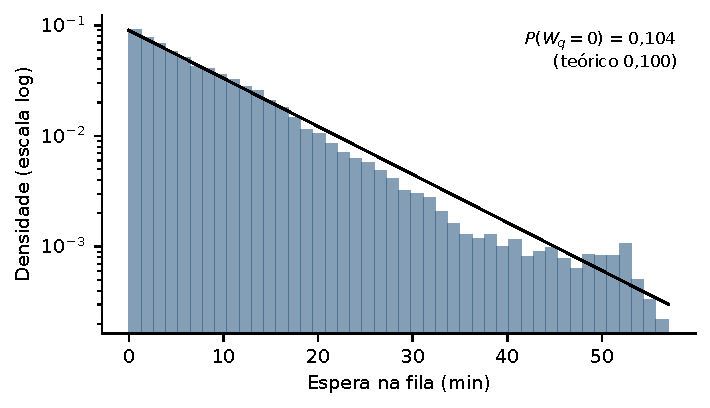
\includegraphics[width=0.62\linewidth]{fig_esperas_individuais}
\figurenote{Histograma das esperas positivas de uma corrida piloto, com escala logarítmica no eixo vertical. A área total é $\rho$, pois a fração restante ($1 - \rho$) tem espera zero. A linha preta é a densidade teórica M/M/1.}
\end{figure}

\begin{figure}[H]
\caption{Distribuição das médias por corrida nas corridas piloto}
\label{fig:medias}
\centering
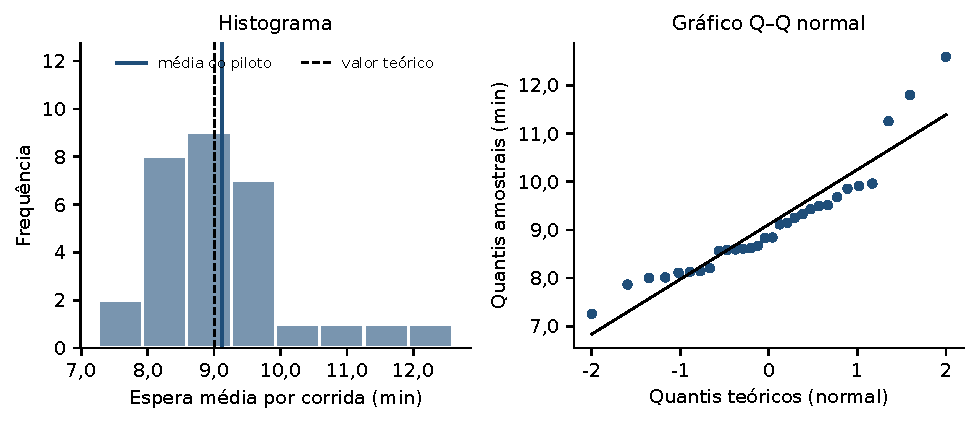
\includegraphics[width=0.95\linewidth]{fig_distribuicao_medias}
\figurenote{Histograma (à esquerda) e gráfico Q--Q normal (à direita) das \RPiloto{} médias por corrida. A linha tracejada é o valor teórico e a linha cheia é a média do piloto.}
\end{figure}

\subsection{Visualizações}
\label{sec:visual}
\paragraph{Independência entre réplicas.}
O projeto exige réplicas independentes.
A Figura~\ref{fig:replicas} mostra as médias por corrida na ordem das réplicas: não há tendência nem agrupamento evidente, e a correlação entre réplicas consecutivas foi $r = \RepLagum{}$ ($p = \RepLagumP{}$), sem indício de dependência (com $n = \RPiloto{}$, o poder é limitado).
Isso é o esperado, porque cada réplica é uma execução completa com semente própria.

\begin{figure}[H]
\caption{Média por corrida segundo a ordem das réplicas piloto}
\label{fig:replicas}
\centering
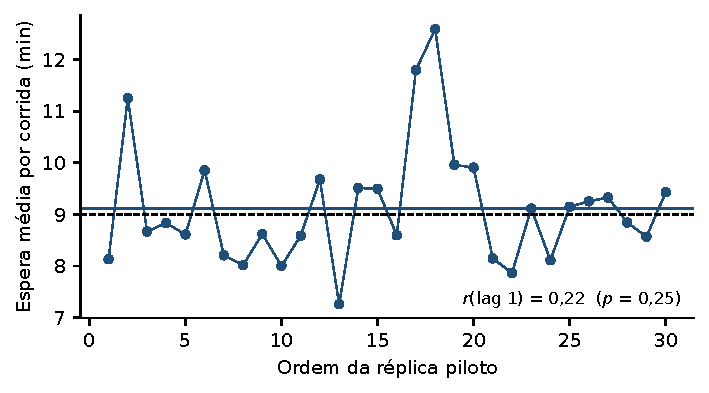
\includegraphics[width=0.7\linewidth]{fig_replicas}
\figurenote{A linha cheia é a média do piloto e a tracejada é o valor teórico. $r$ é a correlação de Pearson entre réplicas consecutivas.}
\end{figure}

\paragraph{Dependência entre clientes.}
As esperas de clientes consecutivos são fortemente correlacionadas: a autocorrelação de defasagem 1 foi \PilotoLagum{} e a de defasagem 10 ainda foi \PilotoLagdez{} (Figura~\ref{fig:acf}).
Portanto, as esperas individuais não são observações independentes.
Por isso a unidade de análise é a média por corrida, e as réplicas do projeto são execuções completas, e não clientes consecutivos nem partes de uma mesma corrida.

\begin{figure}[H]
\caption{Autocorrelação das esperas individuais}
\label{fig:acf}
\centering
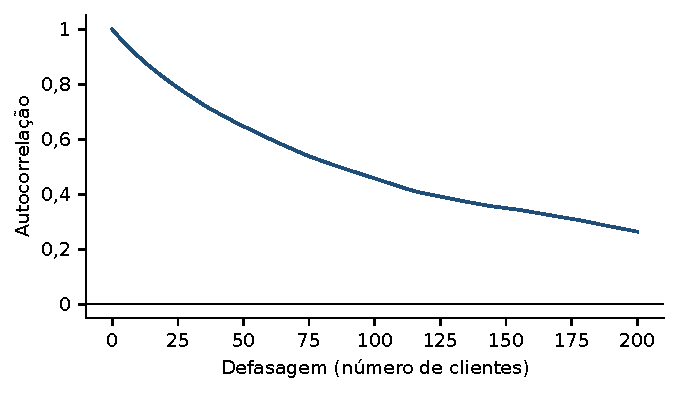
\includegraphics[width=0.7\linewidth]{fig_acf}
\figurenote{Função de autocorrelação amostral das esperas de uma corrida piloto, até a defasagem 200.}
\end{figure}

\paragraph{Período de aquecimento.}
Como o sistema começa vazio, os primeiros clientes esperam menos que os do regime estacionário.
A Figura~\ref{fig:welch} mostra o procedimento gráfico de \textcite{welch1983}: a média entre \RWelch{} réplicas para cada índice de cliente, suavizada por média móvel de \JanelaWelch{} clientes \parencite[ver também][]{law2000,kelton1985}.
A média dos 500 primeiros clientes (\WelchIniMedia{} min) ficou \WelchDifPct{}\% em relação ao platô (\WelchPlatoMedia{} min), e a curva se estabiliza antes de 1.000 clientes.
Com $W = $ \Aquecimento{}, a diferença entre os clientes 1.001 a 2.000 e o platô foi de \WelchResidDif{} $\pm$ \WelchResidEp{} min (erro-padrão), indistinguível de zero.

\begin{figure}[H]
\caption{Procedimento gráfico de Welch para o período de aquecimento}
\label{fig:welch}
\centering
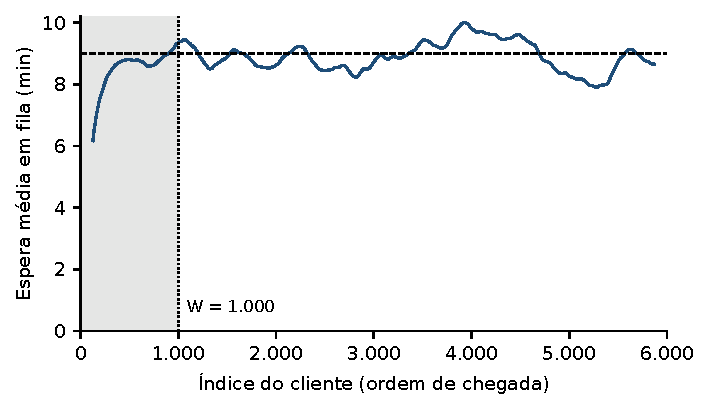
\includegraphics[width=0.7\linewidth]{fig_welch}
\figurenote{Média entre \RWelch{} réplicas de \NWelch{} clientes, suavizada por média móvel de \JanelaWelch{} clientes. A linha tracejada é o valor teórico do regime estacionário; a região cinza é o aquecimento descartado ($W = $ \Aquecimento{}).}
\end{figure}

\subsection{Viabilidade e decisões de projeto}
A Tabela~\ref{tab:comprimento} compara corridas de \NCurto{} e de \NClientes{} clientes.
Com \NCurto{} clientes, o coeficiente de variação foi de \CompCurtoCv{}\%, o que, com $r = 10$, daria um intervalo de confiança de cerca de $\pm$\CompCurtoMeia{}\% sobre a média de uma combinação.
Com \NClientes{} clientes, o coeficiente de variação caiu para \CompLongoCv{}\% ($\pm$\CompLongoMeia{}\%), a um custo de \PilotoTempo{} s por corrida.

\begin{table}[H]
\caption{Efeito do comprimento da corrida sobre a dispersão da resposta}
\label{tab:comprimento}
\begin{tabular}{rrrrr}
\toprule
$N$ (clientes) & $s$ (min) & CV (\%) & Meia-largura do IC ($r=10$) & Tempo/corrida (s) \\
\midrule
10.000 & 1,508 & 17,2 & $\pm$ 12,3\% & 0,088 \\
50.000 & 1,166 & 12,8 & $\pm$ 9,2\% & 0,445 \\
\bottomrule
\end{tabular}

\tablenote{Piloto da célula 3 ($W = $ \Aquecimento{} em ambos os casos), com \RPiloto{} corridas por linha. $s$: desvio-padrão das médias por corrida. CV: coeficiente de variação. Meia-largura do IC: $t_{0{,}975;\,9}\, s / (\sqrt{10}\,\bar{y})$, em porcentagem da média, para uma combinação com $r = 10$ replicações.}
\end{table}

As decisões que decorrem da AED são:
\begin{enumerate}[label=(\arabic*),nosep]
  \item usar $N = $ \NClientes{} clientes por corrida, para reduzir a dispersão da resposta (se a precisão ainda for insuficiente, $N$ ou $r$ podem crescer, pois cada corrida custa menos de 1 s);
  \item descartar $W = $ \Aquecimento{} clientes, valor com margem sobre o ponto em que a curva de Welch se estabiliza;
  \item usar a média por corrida como unidade de análise, com réplicas que são execuções completas e independentes;
  \item verificar no experimento a normalidade e a homogeneidade de variâncias dos resíduos, considerando a transformação logarítmica;
  \item executar as 80 corridas em cerca de \TempoTotalEstimado{} s, tempo compatível com o hardware disponível.
\end{enumerate}

% =====================================================================================
\section{Considerações Finais e Próximos Passos}
% =====================================================================================
O piloto mostrou que o simulador é coerente com a teoria, que o aquecimento e o comprimento das corridas estão bem definidos, que as réplicas são independentes e que a média por corrida é assimétrica à direita, o que exigirá verificar a normalidade e a homogeneidade de variâncias dos resíduos do experimento.
Nada disso avalia a hipótese geral, que depende do fatorial completo.
Os próximos passos, na Entrega 2, são: (a) executar as 80 corridas na ordem aleatória do plano; (b) estimar os efeitos principais e as interações, com intervalos de confiança e testes de significância; (c) verificar as suposições com os resíduos; e (d) fazer a avaliação preliminar da hipótese.

Este estudo tem limitações que devem ser mantidas em mente na interpretação: os resultados valem para chegadas de Poisson, fila infinita e tempo de serviço com média fixa; $r = 10$ é o mínimo exigido, e, como o custo de cada corrida é baixo, o número de replicações pode ser aumentado se os intervalos de confiança ficarem largos; e a combinação com servidor duplo e serviço constante não tem verificação teórica exata.

\printbibliography[title={Referências}]

% =====================================================================================
\appendix
\section{Plano de Aleatorização}
% =====================================================================================
O plano completo das 80 corridas está em \texttt{dados/plano\_experimental.csv}.
Ele é gerado por \texttt{codigo/plano\_experimental.py} com a semente-mestre das corridas ($\texttt{SEED\_EXPERIMENTO} = 20260922$) e a semente da permutação da ordem ($\texttt{SEED\_ORDEM} = 20260923$).
A Tabela~\ref{tab:plano} mostra as primeiras 12 corridas da ordem sorteada.

\begin{table}[H]
\caption{Primeiras corridas da ordem de execução aleatorizada}
\label{tab:plano}
\small
\begin{tabular}{ccccccc}
\toprule
Ordem & Corrida & Célula & Réplica & $c$ & $\lambda$ / Serviço & Chave da semente \\
\midrule
1 & 24 & 3 & 4 & 1 & 0,9 / exponencial & 23 \\
2 & 62 & 7 & 2 & 1 & 0,9 / constante & 61 \\
3 & 56 & 6 & 6 & 2 & 0,5 / constante & 55 \\
4 & 26 & 3 & 6 & 1 & 0,9 / exponencial & 25 \\
5 & 73 & 8 & 3 & 2 & 0,9 / constante & 72 \\
6 & 55 & 6 & 5 & 2 & 0,5 / constante & 54 \\
7 & 53 & 6 & 3 & 2 & 0,5 / constante & 52 \\
8 & 15 & 2 & 5 & 2 & 0,5 / exponencial & 14 \\
9 & 78 & 8 & 8 & 2 & 0,9 / constante & 77 \\
10 & 9 & 1 & 9 & 1 & 0,5 / exponencial & 8 \\
11 & 59 & 6 & 9 & 2 & 0,5 / constante & 58 \\
12 & 71 & 8 & 1 & 2 & 0,9 / constante & 70 \\
\bottomrule
\end{tabular}

\tablenote{A chave da semente identifica o filho de \texttt{SeedSequence.spawn} usado na corrida. O plano completo tem 80 linhas.}
\end{table}

% =====================================================================================
\section{Organização dos Arquivos e Reprodução}
% =====================================================================================
\begin{verbatim}
entrega1/
  codigo/        simulador.py, config.py, piloto_eda.py,
                 plano_experimental.py, verificacao_simulador.py,
                 executar_experimento.py, requirements.txt
  dados/         piloto_*.csv, plano_experimental.csv, verificacao_simulador.csv
  figuras/       figuras em PDF geradas por piloto_eda.py
  tabelas/       tabelas e macros numéricos em LaTeX (gerados)
  relatorio/     relatorio.tex, referencias.bib
  apresentacao/  apresentacao.tex
  Makefile
\end{verbatim}

Para reproduzir os resultados desta entrega: \texttt{pip install -r codigo/requirements.txt}, seguido de \texttt{make all}, que executa o piloto, a verificação do simulador, o plano experimental e compila o relatório e a apresentação.
As 80 corridas do experimento só serão executadas depois da aprovação da proposta, com \texttt{python codigo/executar\_experimento.py}.

\end{document}
